% Template for PLoS
% Version 1.0 January 2009
%
% To compile to pdf, run:
% latex plos.template
% bibtex plos.template
% latex plos.template
% latex plos.template
% dvipdf plos.template

\documentclass[10pt]{article}

% amsmath package, useful for mathematical formulas
\usepackage{amsmath}
% amssymb package, useful for mathematical symbols
\usepackage{amssymb}

% graphicx package, useful for including eps and pdf graphics
% include graphics with the command \includegraphics
\usepackage{graphicx}

% cite package, to clean up citations in the main text. Do not remove.
\usepackage{cite}

\usepackage{color}

% Use doublespacing - comment out for single spacing
\usepackage{setspace}
\doublespacing


% Text layout
\topmargin 0.0cm
\oddsidemargin 0.5cm
\evensidemargin 0.5cm
\textwidth 16cm
\textheight 21cm

% Bold the 'Figure #' in the caption and separate it with a period
% Captions will be left justified
\usepackage[labelfont=bf,labelsep=period,justification=raggedright]{caption}

% Use the PLoS provided bibtex style
\bibliographystyle{plos2009}

% Remove brackets from numbering in List of References
\makeatletter
\renewcommand{\@biblabel}[1]{\quad#1.}
\makeatother


% Leave date blank
\date{}

\pagestyle{myheadings}
%% ** EDIT HERE **


%% ** EDIT HERE **
%% PLEASE INCLUDE ALL MACROS BELOW
\newcommand{\yst}{\ensuremath{y_{st}}}
\newcommand{\tyst}{\ensuremath{\tilde y_{st}}}
\newcommand{\tzs}{\ensuremath{\tilde z_{s}}}
\newcommand{\tzst}{\ensuremath{\tilde z_{st}}}
\newcommand{\zst}{\ensuremath{z_{st}}}
\newcommand{\zs}{\ensuremath{z_{s}}}
\newcommand{\bg}{\ensuremath{\boldsymbol{\gamma}}}
\newcommand{\bxst}{\ensuremath{\mathbf{x}_{st}}}
\newcommand{\bK}{\ensuremath{\mathbf{K}}}
\newcommand{\bn}{\ensuremath{\boldsymbol{\eta}}}
\newcommand{\bb}{\ensuremath{\boldsymbol{\beta}}}
\newcommand{\by}{\ensuremath{\mathbf{y}}}
\newcommand{\bz}{\ensuremath{\mathbf{z}}}
\newcommand{\bX}{\ensuremath{\mathbf{X}}}
\newcommand{\be}{\ensuremath{\boldsymbol{\epsilon}}}
\newcommand{\bQ}{\ensuremath{\mathbf{Q}}}




%% END MACROS SECTION

\begin{document}

% Title must be 150 characters or less
\begin{flushleft}
{\Large
\textbf{A hierarchical modeling framework for the analysis of
multiple-covariate, multiple-observer distance sampling data} }
% Insert Author names, affiliations and corresponding author email.
\\
Paul B. Conn $^{1,\ast}$,
Devin S. Johnson$^{1}$,
Jeffrey L. Laake $^{1}$,
Michael F. Cameron$^{1}$
\\
\bf{1} NOAA National Marine Mammal Laboratory, Alaska Fisheries Science Center,
7600 Sand Point Way NE, Seattle, WA, 98115 U.S.A.
\\
$\ast$ E-mail: paul.conn@noaa.gov
\end{flushleft}

% Please keep the abstract between 250 and 300 words
\section*{Abstract}
We'll do the abstract last...

% Please keep the Author Summary between 150 and 200 words
% Use first person. PLoS ONE authors please skip this step.
% Author Summary not valid for PLoS ONE submissions.
%\section*{Author Summary}

\section*{Introduction}

Distance sampling \cite{BucklandEtAl2001} is often used to estimate the density or abundance of animal populations, and is a central component to many inventory and monitoring programs.  When animals are detectable from the air, from vessels at sea, or by other means (e.g. avian auditory counts), distance sampling provides a means to correct for imperfect detection in animal surveys without having to physically capture and mark animals.  Correcting for imperfect detection is necessary when estimating absolute abundance, and is also viewed by many as an essential component of trend estimation because trends in detectability are typically confounded with trends in abundance unless detectability is explicitly estimated \cite{Buckland2006,NicholsEtAl2009}.  For these reason, practitioners routinely use distance sampling in contemporary transect surveys of marine mammals, sea birds, and passerines.

In it's canonical form (e.g. \cite{BurnhamEtAl1980}), distance sampling may be viewed an extension of strip transect sampling, whereby an observer travels along transects (often selected via systematic sampling), noting the perpendicular distance of groups of animals from the line.  Analysts then fit models to distance data to correct for decreasing detection probabilities as a function of distance from the line, and calculate estimates of animal abundance or density using formulae that correct for average group size, the proportion of area surveyed, and the estimated probability of detection.

Researchers have extended conventional distance sampling to account for a variety of complications that arise in real life sampling scenarios.  Several studies have utilized multiple observers to relax the assumption of 100\% detection on the transect line \cite{BorchersEtAl1998}, or to model heterogeneity in detection as a function of distance \cite{BorchersEtAl2006,BucklandEtAl2010}, both of which cause negative bias in abundance estimates.  Others have accounted and adjusted for the effects of covariates on detection probabilities \cite{DrummerMcdonald1987,RamseyEtAl1987,MarquesBuckland2003}, which can be particularly problematic if associated with individual groups of animals.  For instance, if higher group sizes lead to higher detection probabilities, the mean observed group size will often be higher than the population mean, leading to a positively biased abundance estimator if not explicitly accounted for \cite{DrummerMcdonald1987}.

Conventional, design-based distance sampling estimators are typically obtained via a two step procedure, whereby one first fits a detection function to distance data, and then uses the fitted model to estimate density or abundance over the landscape. Recently, much attention in ecology has been given to incorporating process models for abundance into the estimation process \cite{RoyleEtAl2004,RoyleEtAl2007}.  Spatial autocorrelation is pervasive in ecology, and it's inclusion can permit more precise inferences about abundance because areas with little to no sampling are informed by their neighbors, in effect ``. . .borrowing strength from the ensemble" \cite{Morris1983}.  Including such a model can also permit better inferences about how animal density changes across the landscape. In many cases, inclusion of such a process model requires a shift to a model-based estimation perspective, whereby abundance or some proxy (density, abundance intensity) are estimated simultaneously with parameters of the detection function. Several authors recently modeled spatial dependence when analyzing distance sampling data \cite{HedleyBuckland2004,JohnsonEtAl2010} using point process likelihoods, but we know of no studies which simultaneously consider inclusion of spatial dependence, individual and covariate effects on detection probability, and the ability to incorporate data from multiple observers.

Hierarchical models are a natural framework for simultaneously modeling abundance and detection probabilities, as observation models can be superimposed on an underlying model for abundance intensity.  Moore and Barlow \cite{MooreBarlow2011} recently used a hierarchical model to account for strata and year effects on underlying densities when analyzing line transect data, but did not attempt to model data from multiple observers or use individual covariates in estimation. Likewise, Schmidt et al. \cite{SchmidtEtAl2012} formulated a hierarchical model for single observer distance sampling data using data augmentation within WinBUGS software \cite{LunnEtAl2000}, borrowing ideas popularized in capture-recapture studies \cite{RoyleEtAl2007b,RoyleDorazio2008,Royle2009}.  Previously suggested by several authors for use with distance data \cite{RoyleDorazio2008,LinkBarker2010}, this latter approach has the advantage that individual covariates (such as distance and group size) can be modeled for unobserved groups of animals.
However, this framework incorporates habitat and covariate effects at the level of individual inclusion probabilities (a Bernoulli model is assumed for inclusion of latent groups of animals), which makes it difficult to generalize.  For instance, accommodating transects and grid cells of unequal length is problematic. We argue that incorporating habitat and covariate effects on Poisson (or quasi-Poisson) abundance intensities is a better choice because the Poisson intensity scales linearly with area, making it easy to deal with transects and spatial grid cells that are of different length.

In this paper, we develop hierarchical models for distance sampling data that permit habitat covariates and spatial dependency to influence abundance intensity, while simultaneously modeling effects of covariates on detection probability and permitting multiple observer effects (including ability to have $<$100\% detection on the transect line and to accommodate dependence among observer detections).  At the landscape scale, we employ an intrinsic conditionally autoregressive (ICAR) spatial model \cite{BesagEtAl1991,BesagKooperberg1995,RueHeld2005} to account for habitat covariates and spatial dependency.  Building upon previous work by Durban and Elston \cite{DurbanElston2005} in the context of mark-recapture modeling, our approach for modeling detections and abundance at the transect level is based on data augmentation \cite{TannerWong1987,RoyleEtAl2007b}, using a reversible jump Markov chain Monte Carlo (RJMCMC) algorithm \cite{CarlinChib1995,Green1995} to sample abundance and individual covariates. We provide flexible, user friendly R software for model fitting.

Our modeling approach is applicable to a variety of taxa, but we are particularly motivated by the need to produce density estimates for phocid seals in the Bering Sea.  After describing our proposed model and illustrating it's properties with a simulated dataset, we thus turn our attention to estimating abundance and density of ice seals (bearded, ringed, ribbon, and spotted seals) from helicopter transects conducted in the Bering Sea in 2008.  In addition to group size, we use species as an additional individual covariate on detection probabilities.

% Results and Discussion can be combined.

\section*{Methods}

\subsection*{Hierarchical model}

We propose a hierarchical model for distance sampling data consisting of several conceptually distinct components: a spatial model, an individual covariate model, and an observation model (Figure \ref{fig:DAG}).  Writing the model hierarchically, we can factor these components out
and treat them separately.  Letting the notation $[X]$ define the probability distribution or mass function of $X$, $[X|Y]$ denote the conditional probability of $X$ given $Y$, we (symbolically) write the posterior density of the hierarchical model as follows:
$$
\begin{array}{lll}
[ {\rm Parameters} | {\rm Data}] & \propto & [{\rm Data | Local \hspace{1mm} abundance, Covariates, Detection \hspace{1mm} parameters}]\\
& \times & [{\rm Local \hspace{1mm} abundance | Spatial \hspace{1mm} process}]\\
& \times & [{\rm Covariates|Local \hspace{1mm} abundance, Covariate \hspace{1mm} parameters}]\\
& \times & [{\rm Spatial \hspace{1mm} process | Spatial\hspace{1mm}  parameters}]\\
& \times & [{\rm Prior \hspace{1mm} distributions}]
\end{array}.
$$
In addition, one can make posterior predictions of total abundance, so we might include another component
$[{\rm Abundance |Spatial \hspace{1mm} process,Covariates,Local \hspace{1mm} abundance }]$ as well.
We treat each of these components separately, below.  Notation is largely defined in the text, but is also provided for convenience in Table \ref{tab:defs}.

\subsubsection*{Spatial model}

Previous attempts at incorporating spatial dependence in estimation from line transect data have utilized both (thinned) point process models \cite{HedleyBuckland2004,JohnsonEtAl2010}, and areal spatial models \cite{SchmidtEtAl2012}.  Greater computational efficiency is afforded by choosing an areal spatial model, whereby space is discretized and abundance intensity is treated as constant within each spatial unit.  By it's very nature, this approach leads to a courser spatial surface than point process models, but the degree of courseness can be chosen by the user (e.g., by considering a particular grid granulation).  Given that ecological datasets are typically sparse, we do not expect to lose much precision in inferences about density-habitat relationships from this choice.

Letting $\nu_s$ give the log of abundance intensity at site $s \in {1,2,\hdots,S}$, we impose the following model:
$$
 \boldsymbol{\nu} \sim {\rm Normal}({\bf X}^{\rm hab}
 \boldsymbol{\beta}^{\rm hab}+\boldsymbol{\eta},\tau_\nu^{-1}{\bf I}).
$$
Here, ${\bf X}^{\rm hab}$ gives a design matrix incorporating any predictor variables for abundance, $\boldsymbol{\beta}^{\rm hab}$ gives a vector of regression coefficients, and  $\boldsymbol{\eta}$ denotes a vector of spatial random effects.
The resultant Poisson intensity is then $\lambda_s=A_s \exp(\nu_s)$, where $A_s$ is the relative area of site $s$.  This formulation incorporates habitat covariates in a manner analagous to generalized linear models \cite{McCullaghNelder1989}, but also includes possible spatial autocorrelation and overdispersion relative to the Poisson distribution, two prevalent features of ecological datasets.  In cases where spatial random effects and overdispersion are confounded, one may simply fix $\tau_\nu$ to a large value.

For versatility and ease of implementation, we chose to impose structure on the spatial random effects by means of a \emph{intrinsic conditionally autoregressive} (ICAR) areal spatial model, which is a type of \emph{Gaussian Markov Random Field} \cite{BesagEtAl1991,BesagKooperberg1995,RueHeld2005}.   Specification of an ICAR model starts with articulation of a spatial connectivity matrix, ${\bf C}$.  Let the landscape be discretized into $S$ distinct spatial units (e.g., grid cells).  Then ${\bf C}$ is a $(S \times S)$ dimensional matrix, with $C_{ij}=1$ if spatial unit $i$ is a neighbor of unit $j$, and zero otherwise.  Letting $n_i=\sum_j C_{ij}$ denote the number of neighbors cell $i$ possesses,
we write elements of the precision matrix of the ICAR process ($\bQ$) as
$$
Q_{ij} = \tau_{\rm hab}\left\{\begin{array}{ll}
				-C_{ij} & \mbox{if $i\ne j$}\\
				n_i & \mbox{if $i=j$,}
				\end{array}\right.
$$
where $\tau_{\rm hab}$ is a spatial precision parameter to be estimated.
Given this formulation, the joint probability density function of spatial random effects, $\bn$, is multivariate normal:
$$
[\bn|\tau_{\rm hab}] = {\rm MVN}(\mathbf{0},\bQ^{-1}).
$$
In practice, it is often found that this formulation permits too much flexibility.  In particular, (1) the spatial random effects can be confounded with fixed effect parameters \cite{ReichEtAl2006,HodgesReich2010}, and (2) the spectral decomposition
of $\bQ^{-1}$ permits both positive and negative covariation among spatial grid cells at both fine- and course-scales \cite{HughesHaran2012}.  Our experience is that both of these issues can lead to spuriously high predictions of abundance in grid cells where sampling was never conducted.  Temporarily replacing ${\bf X}^{\rm hab}$ with ${\bf X}$, we reformulate the spatial ICAR model as suggested by Hughes and Haran \cite{HughesHaran2012} and Johnson et al. \cite{JohnsonEtAl2012}, using the following steps:
\begin{enumerate}
 \item Calculate the residual projection matrix, ${\bf P}^\bot = {\bf I}-{\bf X}({\bf X}^\prime{\bf X})^{-1}{\bf X}^\prime$.
 \item Determine the Moran operator matrix, $\boldsymbol{\Omega}=S {\bf P}^\bot {\bf C}{\bf P}^\bot / {\rm sum}({\bf C})$.
 \item Determine the eigenvalues, $\boldsymbol{\lambda}$, and eigenvectors, ${\bf V}$, of $\boldsymbol{\Omega}$.
 \item Use a criterion on $\boldsymbol{\lambda}$ to limit the number of ``effective" spatial random effects.  For instance, limiting ${\bf V}$ to those for which accompanying eigenvalues are greater than 0.5 provides a reasonable level of smoothing \cite{JohnsonEtAl2012}.
 \item Reassemble the selected eigenvectors from ${\bf V}$ into a new, reduced dimensional matrix ${\bf K}$.
 \item Calculate $\boldsymbol{\eta}={\bf K}\boldsymbol{\theta}$, where $[\boldsymbol{\theta}|\tau_{\eta}]= {\rm MVN}({\bf 0},{\bf K}^\prime \bQ {\bf K})$.
\end{enumerate}

\subsubsection*{Local abundance model}
Conditional on $\boldsymbol{\lambda}$ from the spatial abundance process model, we decompose abundance in a given grid cell $s$ into that included in the surveyed area of $s$, and that occurring in the unsurveyed area of $s$.  Let $G_{st}$ represent the number of groups of animals located in $s$ within the area surveyed by transect $t$, and $G_s^*$ be the number of groups located in $s$ outside of the surveyed area.  Then
$$
  G_{st} \sim {\rm Poisson}(P_{st} \lambda_s), \hspace{1mm} {\rm and}
$$
$$
  G_s^* \sim {\rm Poisson}((1-\sum_t P_{st}) \lambda_s).
$$

\subsubsection*{Covariate model}

We model individual covariates as having arisen from a parametric distribution, possibly with overdispersion.  In general, let the covariate
\begin{equation} \label{eq:cov.dist}
x_{ijk} \sim f(g(\theta,\epsilon_{ijk})),
\end{equation}
where $f()$ specifies a probability density or mass function, $g()$ specifies an arbitrary function, $\theta$ gives hyper-priors for $f()$, and $\epsilon_{ijk}$ specify random effects.  We have implemented a number of such functions in our accompanying R package, \emph{dspat}.  For instance, the user can choose $f()$ to be a uniform, multinomial, Poisson, zero-truncated Poisson, overdispersed Poisson, or overdispersed zero-truncated Poisson distribution.  The overdispersed versions of the Poisson distribution are modeled as in \cite{McClintockEtAl2009}; namely
$$
x_{ijk} \sim {\rm Poisson}(\exp(\theta+\sigma \epsilon_{ijk})),
$$
where $\epsilon_{ijk} \sim {\rm Normal}(0,1)$.
The zero-truncated versions of the Poisson distribution are important for modeling covariates such as group size, which are by definition $\ge 1$ \cite{Royle2008}.
One can also choose to fix the parameters of these distributions, or to specify hyper-prior distributions.  For further information, see Dataset S1.

\subsubsection*{Observation (data) model}

Conditional on local abundance and covariates, we assume that observations $Y_{ijk}$ are Bernoulli distributed, with success probabilities $p_{ijk}$.

We model $p_{ijk}$ using a probit link function, expressing them as a function of covariates and including increased dependence among observers as a function of distance.  Assuming two observers,
$$
{\rm probit} \left(\begin{array}{c}
				p_{ij1} \\
				p_{ij2}
		\end{array}\right) \sim {\rm MVN}
\left( \left[ \begin{array}{c}
				{\bf X}_{ij1}^{\rm det} \boldsymbol{\beta}^{\rm det}\\
				{\bf X}_{ij2}^{\rm det} \boldsymbol{\beta}^{\rm det}
		\end{array}\right],
        \left[ \begin{array}{cc}
            1 & \rho_{ij} \\
            \rho_{ij} & 1
        \end{array} \right]
\right),
$$
where $\rho_{ij} = h(d_{ij}) \rho$, $d_{ij}$ is the distance value associated with the $i$th observation in the $j$th transect, and $\rho$ is an estimated parameter.  With binned distance data,
$$
h(d_{ij})=\frac{(d_{ij}-1)}{\max(d_{ij}-1)},
$$
and with unbinned distance data,
$$
h(d_{ij})=\frac{(d_{ij})}{\max(d_{ij})}.
$$
In both cases, $\rho_{ij}$ is assumed to be zero on the line (or in the first distance bin), capturing the essential features of point independence \cite{BorchersEtAl2006,BucklandEtAl2010}.  This formulation allows increased dependence of observations as a function of distance, a common phenomenon in distance sampling.

In practice, an equivalent reparameterization of this model greatly simplifies posterior simulation. In particular, let
\begin{equation} \label{eq:obs.mod}
\left(\begin{array}{c}
				\tilde{Y}_{ij1} \\
				\tilde{Y}_{ij1}
		\end{array}\right) \sim {\rm Normal}
\left( \left[ \begin{array}{c}
				{\bf X}_{ij1}^{\rm det} \boldsymbol{\beta}^{\rm det}\\
				{\bf X}_{ij2}^{\rm det} \boldsymbol{\beta}^{\rm det}
		\end{array}\right],
        \left[ \begin{array}{cc}
            1 & \rho_{ij} \\
            \rho_{ij} & 1
        \end{array} \right]
\right).
\end{equation}
Constraining $Y_{ijk}=1$ if and only if $\tilde{Y}_{ijk}>0$ results in an equivalent probit-Bernoulli model  \cite{AlbertChib1993}.
If there are multiple observers, conditioning on one value of $\tilde{Y}$ reduces the probability density from a bivariate to a univariate distribution.  In particular,
\begin{equation}
\label{eq:biv_to_univ}
[\tilde{Y}_{ij1} | \tilde{Y}_{ij2},\beta^{\rm hab},\rho_{ij}]={\rm Normal}(\mu_{ij1}+\rho_{ij}(\tilde{Y}_{ij2}-\mu_{ij2}),1-\rho_{ij}^2),
\end{equation}
where $\mu_{ijk}={\bf X}_{ijk}^{\rm det} \boldsymbol{\beta}^{\rm det}$.


\subsubsection*{Posterior predictions of abundance}

The model as written focuses on abundance of \emph{groups}.  In contrast, population managers often require estimates of density or abundance that reference the number of unique individuals inhabiting an area of interest.  For the surveyed portion of spatial cells, abundance can simply be calculated as $N_s=\sum_{i=1}^{G_s} n_{is}$, where $n_{is}$ is the group size associated with observation $i$ in cell $s$ (which is itself a modeled covariate).

For unsurveyed portions of spatial cells, abundance $N_s^*$ can be sampled using the parametric model selected for group size.  For the zero-truncated Poisson model,
$$(N_s^*-G_s^*) \sim {\rm Poisson}(\theta G_s^*),
$$
while for the zero-truncated overdispersed Poisson model,
$$(N_s^*-G_s^*) \sim {\rm Poisson}((\theta+0.5\sigma^2) G_s^*).$$
Total abundance is then calculated as $N=\sum_s (N_s+N_s^*)$.

\subsubsection*{Prior distributions}

Bayesian analysis requires specification of prior distributions for $\tau_\eta$, $\tau_\nu$, $\boldsymbol{\beta}^{\rm hab}$, $\boldsymbol{\beta}^{\rm det}$, and $\boldsymbol{\theta}$.  We chose a conjugate ${\rm Gamma}(\alpha,\beta)$ priors for $\tau_\eta$, so that full conditional distributions were available in closed form and could be sampled directly with Gibbs sampling; we chose $\alpha=1$ and $\beta=0.01$ to put ample weight on plausible parameter values. We had difficulty estimating overdispersion and spatial random effects simultaneously, so fix $\tau_\nu=100$ in all applications (though our software includes the capability of specifying a gamma prior for $\tau_\nu$). 

We gave the $\beta$, which are analagous to regression parameters, flat (improper) priors, which is a common strategy in regression problems (e.g., \cite{GelmanEtAl2004}, Chapter 14).  In contrast, we tended to impart more structure to the hyper-priors for individual covariates to improve sampling efficiency.  In our two subsequent examples, we incorporated a ${\rm Gamma}(1.1,1.0)$ distribution for the log of group size, and a ${\rm Uniform}(0,1)$ distribution for $\sigma$ (the standard deviation for log group size random effects); for the ice seal example, species was modeled with a Dirichlet(10,10,10,10,10) distribution, the conjugate prior for the categorical distribution.  Pilot analyses suggested little sensitivity of results to our choice of prior distributions.

\subsection*{Data augmentation and Bayesian inference}

As suggested previously, the primary challenge in implementing a complete data model for multiple covariate distance sampling was in jointly sampling abundance and individual covariates.  We chose to implement a reversible-jump ``Rasch" type model for abundance at the transect level, in a manner similar to Durban and Elston \cite{DurbanElston2005}.  This approach consists of several steps, including (1) additions and deletions of unobserved animals to the population, and (2) resampling of covariate values for unobserved animals, and (3) sampling of $\tilde{Y}$ values for new additions. These steps were conducted independently for each transect; thus without loss of generality, we present sampling details for a single transect. We also assume that each transect is conducted within a single spatial grid cell with abundance intensity $\lambda_j$ (in practice, transects spanning multiple cells can be broken into multiple, independent transects and treated separately).

Specification of the complete data model starts with specifying an integer $M_j$ that serves as the upper limit for the number of groups of animals present in the sampled area of transect $j$. In practice, this integer can be increased if it is found that the posterior group abundance runs up against this bound \cite{DurbanElston2005,RoyleEtAl2007b}. However, choosing too large of a value can dramatically increase computing time.

Addition and deletion steps consist of increasing or decreasing the value of $G_j$, and are accomplished as follows:
\begin{itemize}
    \item Propose a new value for $G_j$, $G_j^\prime=G_j+u$, where
    $u\sim {\rm Uniform}(-a,a)$, where $a$ is a tuning parameter set to achieve a target acceptance rate of 0.3-0.4.
    \item Accept proposal with probability $r$, where
    $$
    r= \left\{ \begin{array}{lll}
				\lambda_j^u \prod_{i=1}^u
                \frac{1-p_{G_j+i,j}}{G_j-G_j^{\rm obs}+i}& & u>0\\
			    \lambda_j^u \prod_{i=1}^{-u}
                \frac{G_j-G_j^{\rm obs}-i+1}{
                1-p_{G_j-i+1,j}}& & u<0
		\end{array}. \right.
    $$
\end{itemize}
    Here, $p_{ij}$ equals the probability that group $i$ of transect $j$ is observed by one or more observer.  If there is only one observer on transect $j$, this probability is simply $$
      p_{ij} = \int_0^\infty {\rm Normal}(x;{\bf X}_{ij1}\boldsymbol{\beta}^{\rm det},1)dx;
    $$
    if $O_j=2$,
    $$
      p_{ij} = \int_0^\infty \int_0^\infty {\rm Normal}
        \left( \left[ \begin{array}{c}
				x\\
				y
		\end{array} \right]; \left[
        \begin{array}{c}
				{\bf X}_{ij1}^{\rm det} \boldsymbol{\beta}^{\rm
                det}\\
				{\bf X}_{ij2}^{\rm det} \boldsymbol{\beta}^{\rm
                det}
		\end{array}\right],
        \left[ \begin{array}{cc}
            1 & \rho_{ij} \\
            \rho_{ij} & 1
        \end{array} \right]
        \right) dx dy
    $$

These Metropolis ratios follow directly from a sampling model where the likelihood of observing $G_j^{\rm obs}$ individuals out of $G_j$ total animals is
$$
\left( \begin{array}{l}
G_j \\
G_j^{\rm obs}
\end{array} \right)
\prod_{i=1}^{G_j} p_{ij}^{Y_{ij}} (1-p_{ij})^{(1-Y_{ij})},
$$
where $Y_{ij}=\max(Y_{ij1},Y_{ij2})$.  Link and Barker \cite{LinkBarker2010} used a similar model formulation in their complete data representation of distance data.

Following the addition/deletion step, the next step in our RJMCMC estimation scheme is to resample individual covariates.  For each such covariate, there are two categories of values to update: (1) covariates for which a group of animals were in the population and never observed, and (2) latent groups not currently belonging to the population. Letting $G_j^{\rm obs}$ denote the number of groups observed by at least one observer in transect $j$, and $G_j$ be the total number of groups for transect $j$ at the previous iteration of the Markov chain, the full conditional distribution for a given covariate $c$, $x_{ijc}$ is given by
$$
[Y_{ij1}=0,Y_{ij2}=0|{\bf x}_{ij},\boldsymbol{\beta},{\bf X}_{ij1},{\bf X}_{ij2}]][x_{ijc}|\boldsymbol{\theta}],
$$
for $i \in (G_i^{\rm obs}+1,G_{j}^{\rm obs}+2,\hdots,G_j)$, 
which is just the observation model (e.g. Eq. \ref{eq:obs.mod}) multiplied by the prior distribution of the individual covariate.  We use a Metropolis-Hastings step to sample from this distribution.

For groups $G_j+1,G_j+2, \hdots,M$ (i.e., ``pseudo-animals" not in the population), we simulate covariates directly from Eq. \ref{eq:cov.dist}.  These distributions are used in place of the pseudo-prior distributions suggested by Durban and Elston \cite{DurbanElston2005}.  The difference between our approaches is that in the present work we obtain posterior samples of the parameters specified in  $f()$ (e.g., the parameters describing the underlying covariate distribution), while Durban and Elston fix these parameters.  Simulations (see below) suggest that this approach results in estimates with reasonable properties, and also bypasses the need to tediously tune pseudo-prior distributions.  Conforming to a priori expectations, we used a uniform distribution for simulation of pseudo-animal distances (note that simulating from $[d_{ij} | Y_{ijk}=0]$ instead leads to positively biased abundance estimates!).

Estimation of remaining model parameters (conditional on a set level of abundance)  proceeded by cyclical sampling of model parameters from their full conditional distributions \cite{GelmanEtAl2004}.  In particular, we employed a combination of Gibbs, Metropolis-Hastings, and Langevin-Hastings \cite{RobertCasella2004} steps for posterior simulation.  For Metropols-Hastings steps, candidate parameter values were sampled from uniform distributions centered at the previous iterations parameter value and with a range chosen to achieve an acceptance rate of 30-40\% as suggested by Gelman Et Al. \cite{GelmanEtAl2004}.  For Langevin-Hastings steps, proposal vectors depended on the parameter vector at the previous iteration, as well as the gradient of the joint full conditional distribution evaluated at the current set of parameter values.

\subsubsection*{Sampling $\boldsymbol{\beta}^{\rm hab}$}

The full conditional distribution for $[\boldsymbol{\beta}^{\rm hab}|\hdots]$ (the conditional distribution of $\boldsymbol{\beta}^{\rm hab}$ given all other parameters is given by
$$
    [\boldsymbol{\nu} | \boldsymbol{\beta}^{\rm hab},{\bf X}^{\rm hab},\boldsymbol{\eta},\tau_\nu][\boldsymbol{\beta}^{\rm hab}]\propto[\boldsymbol{\nu} | \boldsymbol{\beta}^{\rm hab},{\bf X}^{hab},\boldsymbol{\eta},\tau_\nu],
$$
where $ [\boldsymbol{\nu} | \boldsymbol{\beta}^{\rm hab},{\bf X}^{\rm hab},\boldsymbol{\eta},\tau_\nu]$
is the product normal likelihood
\begin{equation} \label{eq:nu.lik}
{\rm Normal}(\boldsymbol{\nu};{\bf X}^{\rm hab} \boldsymbol{\beta}^{\rm hab} +\boldsymbol{\eta},\tau_\nu^{-1}{\bf I}).
\end{equation}
Rewriting Eq. \ref{eq:nu.lik} as
$$
{\rm Normal}(\boldsymbol{\nu}-\boldsymbol{\eta};{\bf X}^{\rm hab}\boldsymbol{\beta}^{\rm hab} ,\tau_\nu^{-1}{\bf I})
$$
makes it into a standard linear regression formula. We may
thus use Gibbs sampling to sample directly from $[\boldsymbol{\beta}^{\rm hab}|\hdots]$ (e.g. \cite{GelmanEtAl2004}, chapter 14), using
\begin{equation}
\label{eq:beta.post}
[\boldsymbol{\beta}^{\rm hab}|\hdots]={\rm Normal}(({\bf X}^\prime {\bf X})^{-1}{\bf X}^\prime (\boldsymbol{\nu}-\boldsymbol{\eta}),\tau_\nu^{-1}({\bf X}^\prime {\bf X})^{-1})
\end{equation}
(temporarily replacing ${\bf X}^{\rm hab}$ with ${\bf X}$).

\subsubsection*{Sampling $\boldsymbol{\eta}$}

We employ a similar strategy to sample from  $[\boldsymbol{\eta}|\hdots]$.  In this case, we
rewrite Eq. \ref{eq:nu.lik} as
$$
{\rm Normal}(\boldsymbol{\nu}-{\bf X}^{\rm hab}\boldsymbol{\beta}^{\rm hab};\boldsymbol{\eta} ,\tau_\nu^{-1}{\bf I}).
$$
Here, the ``data" are $(\boldsymbol{\nu}-{\bf X}^{\rm hab}\boldsymbol{\beta}^{\rm hab})$, while the regression parameters are $\boldsymbol{\eta}$ with an identity design matrix. In application without spatial restriction of random effects, the prior precision of $\boldsymbol{\eta}$ is ${\bf Q}^{-1}$, so that
$$
[\boldsymbol{\eta}|\hdots] = {\rm Normal}(\Sigma_\eta \tau_\nu (\boldsymbol{\nu}-{\bf X}^{\rm hab}\boldsymbol{\beta}^{\rm hab}),\Sigma_\eta),
$$
where
$$
\Sigma_\eta=(\tau_\nu{\bf I} + {\bf Q})^{-1}.
$$
This distribution may be sampled directly via Gibbs sampling. Owing to the sparse nature of $\bQ$, we increased computational efficiency by utilizing numerical routines specifically formulated for sparse matrices (see Dataset S1).

In applications with spatial restriction, $\boldsymbol{\eta} = {\bf K}\boldsymbol{\theta}$, so we instead need to sample $\boldsymbol{\theta}$.  In this case, we redefine the precision matrix of the ICAR process as ($\bQ_\theta={\bf K}^\prime \bQ {\bf K}$), and write the full conditional distribution for $\boldsymbol{\theta}$ as
$$
[\boldsymbol{\theta}|\hdots] = {\rm Normal}(\Sigma_\theta {\bf K}^\prime (\boldsymbol{\nu}-{\bf X}^{\rm hab}\boldsymbol{\beta}^{\rm hab}),\Sigma_\theta),
$$
where $\Sigma_\theta=({\bf K}^\prime {\bf K} + {\bf Q_\theta})^{-1}$ \cite{HughesHaran2012,JohnsonEtAl2012}.

 

\subsubsection*{Sampling $\tau_\eta$}
Given a $\textrm{Gamma}(\alpha_\eta,\beta_\eta)$ prior, $\tau_\eta$ may be directly sampled using
$$
\tau_\eta \sim \textrm{Gamma}\left( 0.5(S-1)+\alpha_\eta,0.5\boldsymbol{\eta}^\prime {\bf Q} \boldsymbol{\eta}+\beta_\eta \right).
$$
When spatial restriction is employed, 
$$
\tau_\eta \sim \textrm{Gamma}\left( 0.5(n-1)+\alpha_\eta,0.5\boldsymbol{\theta}^\prime \bQ_\theta \boldsymbol{\theta} +\beta_\eta \right),
$$
where $n$ gives the length of $\boldsymbol{\theta}$.

\subsubsection*{Sampling $\boldsymbol{\nu}$}
We simultaneously updated the entire vector $\boldsymbol{\nu}$ using a Langevin-Hastings algorithm \cite{RobertCasella2004}.  The Langevin-Hastings algorithm utilizes the numerical gradient of the full conditional distribution to make more efficient proposals, which are accepted or rejected based on a modified Metropolis ratio.  The full conditional distribution for $\boldsymbol{\nu}$ needed to perform Langevin-Hastings updates is given by
$$
\left[ \boldsymbol{\nu} | \hdots \right] = \textrm{Normal}\left(\boldsymbol{\nu};{\bf X}^{\rm hab}\boldsymbol{\beta}^{\rm hab}+\boldsymbol{\eta},\tau_\nu^{-1} {\bf I} \right) \prod_{i=1}^S \textrm{Poisson} \left( G_i; \exp(\nu_i) \right),
$$
where {\bf I} is the $S\times S$ identity matrix.

\subsubsection*{Sampling $\tau_\nu$}
As with $\tau_\eta$, $\tau_\nu$ may be directly sampled using
$$
\tau_\nu \sim \textrm{Gamma}\left( 0.5S+\alpha_\nu,0.5\boldsymbol{\mu}_\nu^\prime \boldsymbol{\mu}_\nu+\beta_\nu \right),
$$
where $\boldsymbol{\mu}_\nu={\bf X}^{\rm hab}\boldsymbol{\beta}^{\rm hab}+\boldsymbol{\eta}$.

\subsubsection*{Sampling $\boldsymbol{\beta}^{\rm det}$}

Using Eq. \ref{eq:biv_to_univ} to transform bivariate responses into univariate responses when necessary, i.e.,
$$
\acute{Y}_{ijk}=
    \left\{ \begin{array}{lll}
				\tilde{Y}_{ijk} & & O_j=1\\
			    \tilde{Y}_{ijk}-\rho_{ij}\tilde{Y}_{ij,3-k} & & O_j=2
		\end{array}, \right.
$$
we loosely arrive at the model
$$
\acute{{\bf Y}} \sim {\rm Normal}({\bf X} \boldsymbol{\beta}^{\rm det},\boldsymbol{\Sigma}),
$$
where ${\bf X}={\bf X}^{\rm det}$ if $O_j=1$ and
$$
{\bf X}=\left[ \begin{array}{l}
    {\bf X}_1^{\rm det} - \rho {\bf X}_2^{\rm det} \\
    {\bf X}_2^{\rm det} - \rho {\bf X}_1^{\rm det}
    \end{array}
    \right]
$$
if $O_j=2$ (Here, ${\bf X}_k^{\rm det}$ designates the design matrix for the $k$th observer).
Also, $\boldsymbol{\Sigma}$ is a diagonal matrix with entries corresponding to $1-\rho_{ij}^2$ for each response variable.  Under this formulation, we can use basic Gibbs sampling for regression with a known covariance matrix (e.g., \cite{GelmanEtAl2004}, Eqs. 14.11-14.12) to sample from $[\boldsymbol{\beta}^{\rm det}|\hdots]$.  In particular,
$$
[\boldsymbol{\beta}^{\rm det}|\hdots]=\textrm{Normal}\left( ({\bf X}^\prime \boldsymbol{\Sigma}^{-1} {\bf X})^{-1}{\bf X}^\prime \boldsymbol{\Sigma}^{-1} \acute{{\bf Y}},
({\bf X}^\prime \boldsymbol{\Sigma}^{-1} {\bf X})^{-1} \right).
$$



\subsubsection*{Sampling $\rho$}

Letting $\xi$ denote the set of transects for which $O_j=2$ (i.e., the set for which there were two observers present), we used a Metropolis-Hastings step to update $\rho$.  The full conditional distribution for this update is given by
$$
  [\rho|\hdots] \propto \left[ \prod_{j \in \xi} \prod_{i=1}^{G_{ij}}
  \{
(1-\rho_{ij}^2)\exp\left(
(1-\rho_{ij}^2)^{-1} (\Delta_{ij1}^2+\Delta_{ij2}^2-2\rho_{ij}\Delta_{ij1}\Delta_{ij2})
  \right)
  \}
  \right]^{-0.5},
$$
where $\Delta_{ijk}=\tilde{Y}_{ijk}-[{\bf X}^{\rm det} \boldsymbol{\beta}]_{ijk}$.

\subsubsection*{Sampling $\tilde{\bf Y}$}

For animals currently in the population (i.e., for $i \in [1,2,\hdots,G_j]$), the full conditional distribution $[ \tilde{Y}_{ijk} | \hdots]$ is a truncated normal, and may be sampled directly.  If $Y_{ijk}=0$, $\tilde{Y}_{ijk}$ is drawn from a normal distribution with the constraint that $\tilde{Y}_{ijk}<0$, while $\tilde{Y}_{ijk}>0$ if $Y_{ijk}=1$.  The corresponding untruncated distribution is given by
$$
\tilde{Y}_{ijk} \sim \textrm{Normal} \left( [{\bf X}^{\rm det} \boldsymbol{\beta}^{\rm det}]_{ijk},1  \right)
$$
when $O_j=1$, and
$$
\tilde{Y}_{ijk} \sim \textrm{Normal} \left( [{\bf X}^{\rm det} \boldsymbol{\beta}^{\rm det}]_{ijk}+\rho_{ij}(\tilde{Y}_{ij,3-k}-[{\bf X}^{\rm det} \boldsymbol{\beta}^{\rm det}]_{ij,3-k}),1-\rho_{ij}^2  \right)
$$
when $O_j=2$.

\subsubsection*{Sampling $\boldsymbol{\theta}, \boldsymbol{\epsilon}$}

If random effects are not specified (i.e., $\epsilon_{ijk}=0$ $\forall$ $\{i,j,k\}$), specification of conjugate priors for the Poisson, zero-truncated Poisson, and multinomial distributions meant that full conditionals were available in closed form and could be simulated directly.  If random effects are specified, both the parameters of the underlying distribution (i.e., $\boldsymbol{\theta}$) and the random effects themselves (i.e., $\boldsymbol{\epsilon}$)
are sampled via the Metropolis-Hastings algorithm.  Owing to the relatively large number of individual covariate distributions, we refer the reader to Dataset S1 for further details.

\subsubsection*{Computing}

We developed generalized computing code to conduct MCMC estimation, which we implemented in the R programming environment \cite{RTeam2007}.  This code has been incorporated into the R package, \emph{dspat} \cite{JohnsonEtAl2010}.  The package, which includes code, help files, and an example analysis, is available as Dataset S1.

\section*{Examples}

\subsection*{Simulated data}

We generated a simulated dataset and analyzed it with our hierarchical model to ensure that model parameters could be properly identified and that abundance estimates were reasonable.  The log of abundance intensity was simulated on a 15 by 15 grid assuming a positive relationship with latitude and spatially correlated error induced via an ICAR process with precision parameter $\tau_\nu=15$ (Fig. \ref{fig:sim_landscape}).  A total of 15 transects were simulated at the longitudinal midpoints of grid cells; latitudinal placement was uniformly distributed   The width of each transect was assumed to encompass 25\% of each grid cell.

After laying down virtual transects, we simulated group abundance and species composition for each transect-grid cell combination.  The group size for group $i$ of transect $j$ was set to $(1+W_{ij})$, where $W_{ij} \sim \textrm{Poisson}(3)$, while species was drawn from a $\textrm{multinomial}(0.1,0.2,0.3,0.4)$ distribution (assuming four possible species).
Detection data were simulated by applying an assumed detection function that was a function of multiple covariates.  Odd numbered transects were allotted two observers, while even numbered transects were allotted one observer; in all cases, observers were picked randomly from a pool of 3 total observers with different underlying detection probabilities.  The assumed detection function was made to be a function of observer, distance, species, and group size.  If multiple observers were present, correlation between observers was modeled as a linearly increasing function of distance on the probit scale, with a maximum value of 0.5 (at the farthest distance bin).  Distances were recorded as one of 5 equally spaced bins.

\subsection*{Ice seals in the Bering Sea}

We collected data from line transect seal surveys conducted from a ??? helicopter operating from the U.S. Coast Guard icebreaker {\it Polar Sea} in June and July, 2008 (?).  The helicopter crew consisted of a pilot and three observers; two of the observers were located on the right (?) side of the vessel, thus providing double observer data, while another observer searched for seals on the left side of the plane.

Need more help here on distance sampling protocols used...(distance bins, etc.)

Section on environmental covariates used (latitude, longtitude?)


\section*{Discussion}

In practice, the parameterization chosen for data augmentation at the transect level may have some real ramifications for scaling up to abundance on the landscape scale.  A limiting case in spatial models is that counts (e.g., abundances in given cells) are distributed according to a Poisson distribution.  The Poisson distribution has the convenient property of proportional scaling.  For example, if abundance in as area $\mathcal{A}$  can be assumed to follow a ${\rm Poisson}(\lambda)$ distribution, then abundance in a smaller area, say $a \in \mathcal{A}$, can be assumed to follow an ${\rm Poisson}(a\lambda)$ distribution.  If $a$ is the proportion of a grid cell covered by a distance sampling transect, there is a direct link between abundance intensity at the landscape level, and that being estimated for each transect.  As we have shown in this paper, this relationship can be incorporated with relative ease using a data augmentation parameterization analagous to that considered by Durban and Elston \cite{DurbanElston2005} for mark-recapture data. In contrast, the approach advocated by Royle and Dorazio \cite{RoyleDorazio2008} and Link and Barker \cite{LinkBarker2010} requires use of an occupancy parameter, $\psi$, the interpretation of which requires reference to the value of $M$ assumed in the model (e.g., $\psi=a\lambda/M$.  Further, the variance of expected abundance in this model (e.g., ${\rm Var}(G)=\psi (1-\psi)/M = a\lambda-a^2\lambda^2$) is negatively biased with regard to the Poisson variance (i.e., ${\rm Var}(G)=a\lambda$).  What effect this has on conducting hierarchical inference on abundance is presently unknown, but was the primary motivation for us choosing the Durban and Elston \cite{DurbanElston2005} parameterization.


% Do NOT remove this, even if you are not including acknowledgments
\section*{Acknowledgments}


%\section*{References}
% The bibtex filename
\bibliography{master_bib}
\clearpage

%\section*{Figures}
%\begin{figure}[!ht]
%\begin{center}
%%\includegraphics[width=4in]{figure_name.2.eps}
%\end{center}
%\caption{
%{\bf Bold the first sentence.}  Rest of figure 2  caption.  Caption
%should be left justified, as specified by the options to the caption
%package.
%}

\begin{figure}
\begin{center}
\includegraphics[width=0.95\textwidth]{DAG.eps}
\end{center}
\caption{{\bf Directed, acyclic graph (DAG) of the (areal) hierarchical model
for distance data}. Individual nodes indicate a parameter or vector of parameters, and arrows represent conditional dependence. Notation is defined in Table \ref{tab:defs}.}
\label{fig:DAG}
\end{figure}
\clearpage

\begin{figure}
\begin{center}
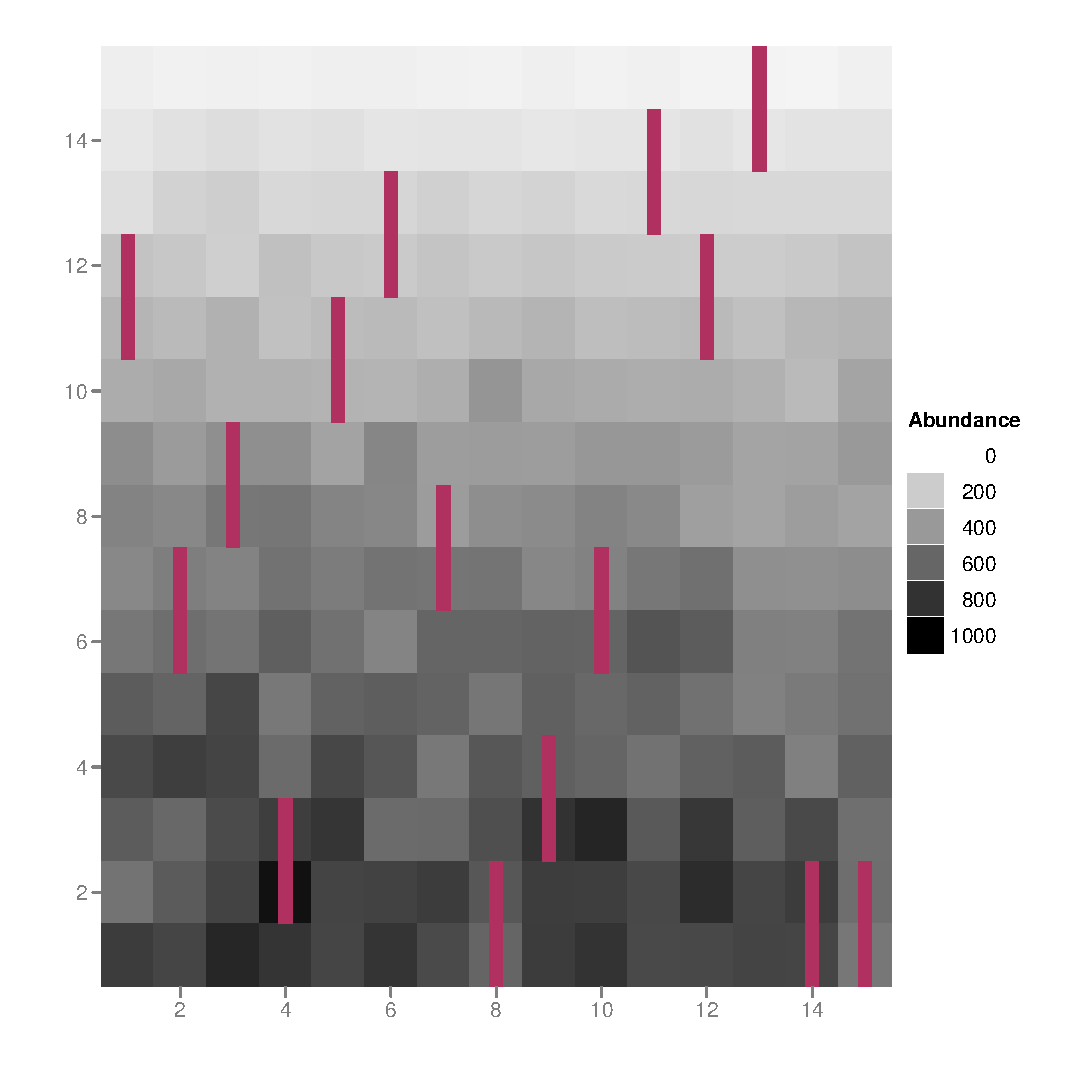
\includegraphics[width=0.95\textwidth]{sim_habitat_true.eps}
\end{center}
\caption{{\bf Simulated abundance over a landscape used for calibrating hierarchical distance sampling model}.  Vertical transects are superimposed, and are assumed to cover 1/4 of the area of each grid cell they intersect.}
\label{fig:sim_landscape}
\end{figure}
\clearpage

\section*{Tables}

\begin{table}
\caption{\bf Parameter and data definitions.}
\begin{tabular}{p{1.5cm}l p{12.5cm}}
\hline \hline \\
& & \\
Parameter & & Definition \\
\cline{1-1} \cline{3-3}
& & \\
$N$ & & Abundance of the focal taxa over the landscape of interest\\
$G_s^*$ & & Number of groups of animals located in unsurveyed regions of spatial cell $s$\\
$G_{st}$   & & Number of groups of animals located in the region of spatial cell $s$ by transect $t$\\
$\nu_{s}$ & & The log of abundance intensity in strata $s$\\
$\tau_\nu$ & & Precision of log of abundance intensity; used to impart overdispersion relative to the Poisson distribution \\
$\lambda_{s}$ & & Abundance intensity in strata $s$ ($=\exp(\nu_s)$)\\
$\boldsymbol{\beta}^{\rm hab}$ & & Parameters of the linear predictor describing variation in
        the log of abundance intensity as a function of habitat covariates\\
$\eta_s$ & & Spatial random effect associated with strata $s$\\
$\tau_\eta$ & & Precision parameter for the spatial ICAR process model\\
$x_{ijk}$   & &  The value of the $k$th individual covariate associated with
    group $i$ in transect $j$ (for groups of animals never observed)\\
$\boldsymbol{\theta}$ & & Parameters describing the distribution of individual covariates
                          at the population level \\
$\epsilon_{ijk}$ & & Random effect associated with the value of the $k$th covariate of the
                $i$th group located in the area surveyed by transect $j$ (assumed Normal(0,1))\\
$\boldsymbol{\beta}^{\rm det}$ & & Parameters of the linear predictor describing variation
        in the probit of detection probability as a function of observer and individual covariates \\
$\rho$ & & Parameter describing increasing correlation between $Y_{ij1}$ and $Y_{ij2}$ as a function of distance in the case of double observer data\\
Data & & Definition \\
\cline{1-1} \cline{3-3}
$Y_{ijk}$ &  & Bernoulli response variable for whether the $i$th group in the $j$th transect
                was observed by observer $k$\\
$G_j^{\rm obs}$ & & Number of groups observed by at least one observer during transect $j$\\
$O_j$   & & Number of observers present when sampling transect $j$ \\
$x_{ijk}$   & &  The value of the $k$th individual covariate associated with group
                $i$ in transect $j$ that were actually observed\\
$w_{jk}$ & & Additional covariates associated with observer $k$ in transect $j$ (e.g.,
            visibility, seat, observer ID)\\
$X^{\rm hab}$   & &  Design matrix associated with habitat model\\
$X^{\rm det}_{ijk}$   & &  Design matrix associated with the detection model for the $i$th group in the $j$th transect
                and observer $k$ (note dependence on
                $w_{jk}$ and $x_{ijk}$) \\
$A_s$   & & The proportional area of strata $s$ relative to mean strata area\\
$P_{st}$   & & The proportion of area in strata $s$ that is surveyed by transect $t$\\
${\bf C}$ & & Binary spatial connectivity matrix, with $C_{ij}=1$ if cells $i$ and $j$ are neighbors, and 0 otherwise\\
$n_s$   & & Number of neighbors cell $s$ has\\
\hline
\end{tabular}
\begin{flushleft}Parameters and data used in the hierarchical model for distance data
\end{flushleft}
\label{tab:defs}
\end{table}

%\begin{table}[!ht]
%\caption{
%\bf{Table title}}
%\begin{tabular}{|c|c|c|}
%table information
%\end{tabular}
%\begin{flushleft}Table caption
%\end{flushleft}
%\label{tab:label}
% \end{table}

\end{document}

